% !TeX root = ../../thesis.tex

\subsection{\tcs{}}
The second algorithm closely resembles the previous one. Instead of determining the minimal hitting set of the test suite in order to permanently remove tests, this algorithm has a notion of context. Prior to the execution of the tests, the algorithm performs a \emph{white-box static analysis} of the codebase to identify which parts have been changed. Subsequently, only the tests regarding modified parts are executed, making the selection temporary (\autoref{fig:tcs}) and modification-aware \cite{10.1002/stv.430}. Rothermel and Harrold define this formally in \autoref{def:tcs}.

\begin{definition}[\tcs{}]
\label{def:tcs}
\mbox{}\\Given:
\begin{itemize}
	\item $P$ the previous version of the codebase
	\item $P'$ the current (modified) version of the codebase
	\item $T$ the test suite
\end{itemize}

\noindent \tcs{} aims to find a subset $T' \subseteq T$ that is used to test $P'$. 
\end{definition}

\begin{figure}[htbp!]
	\centering
	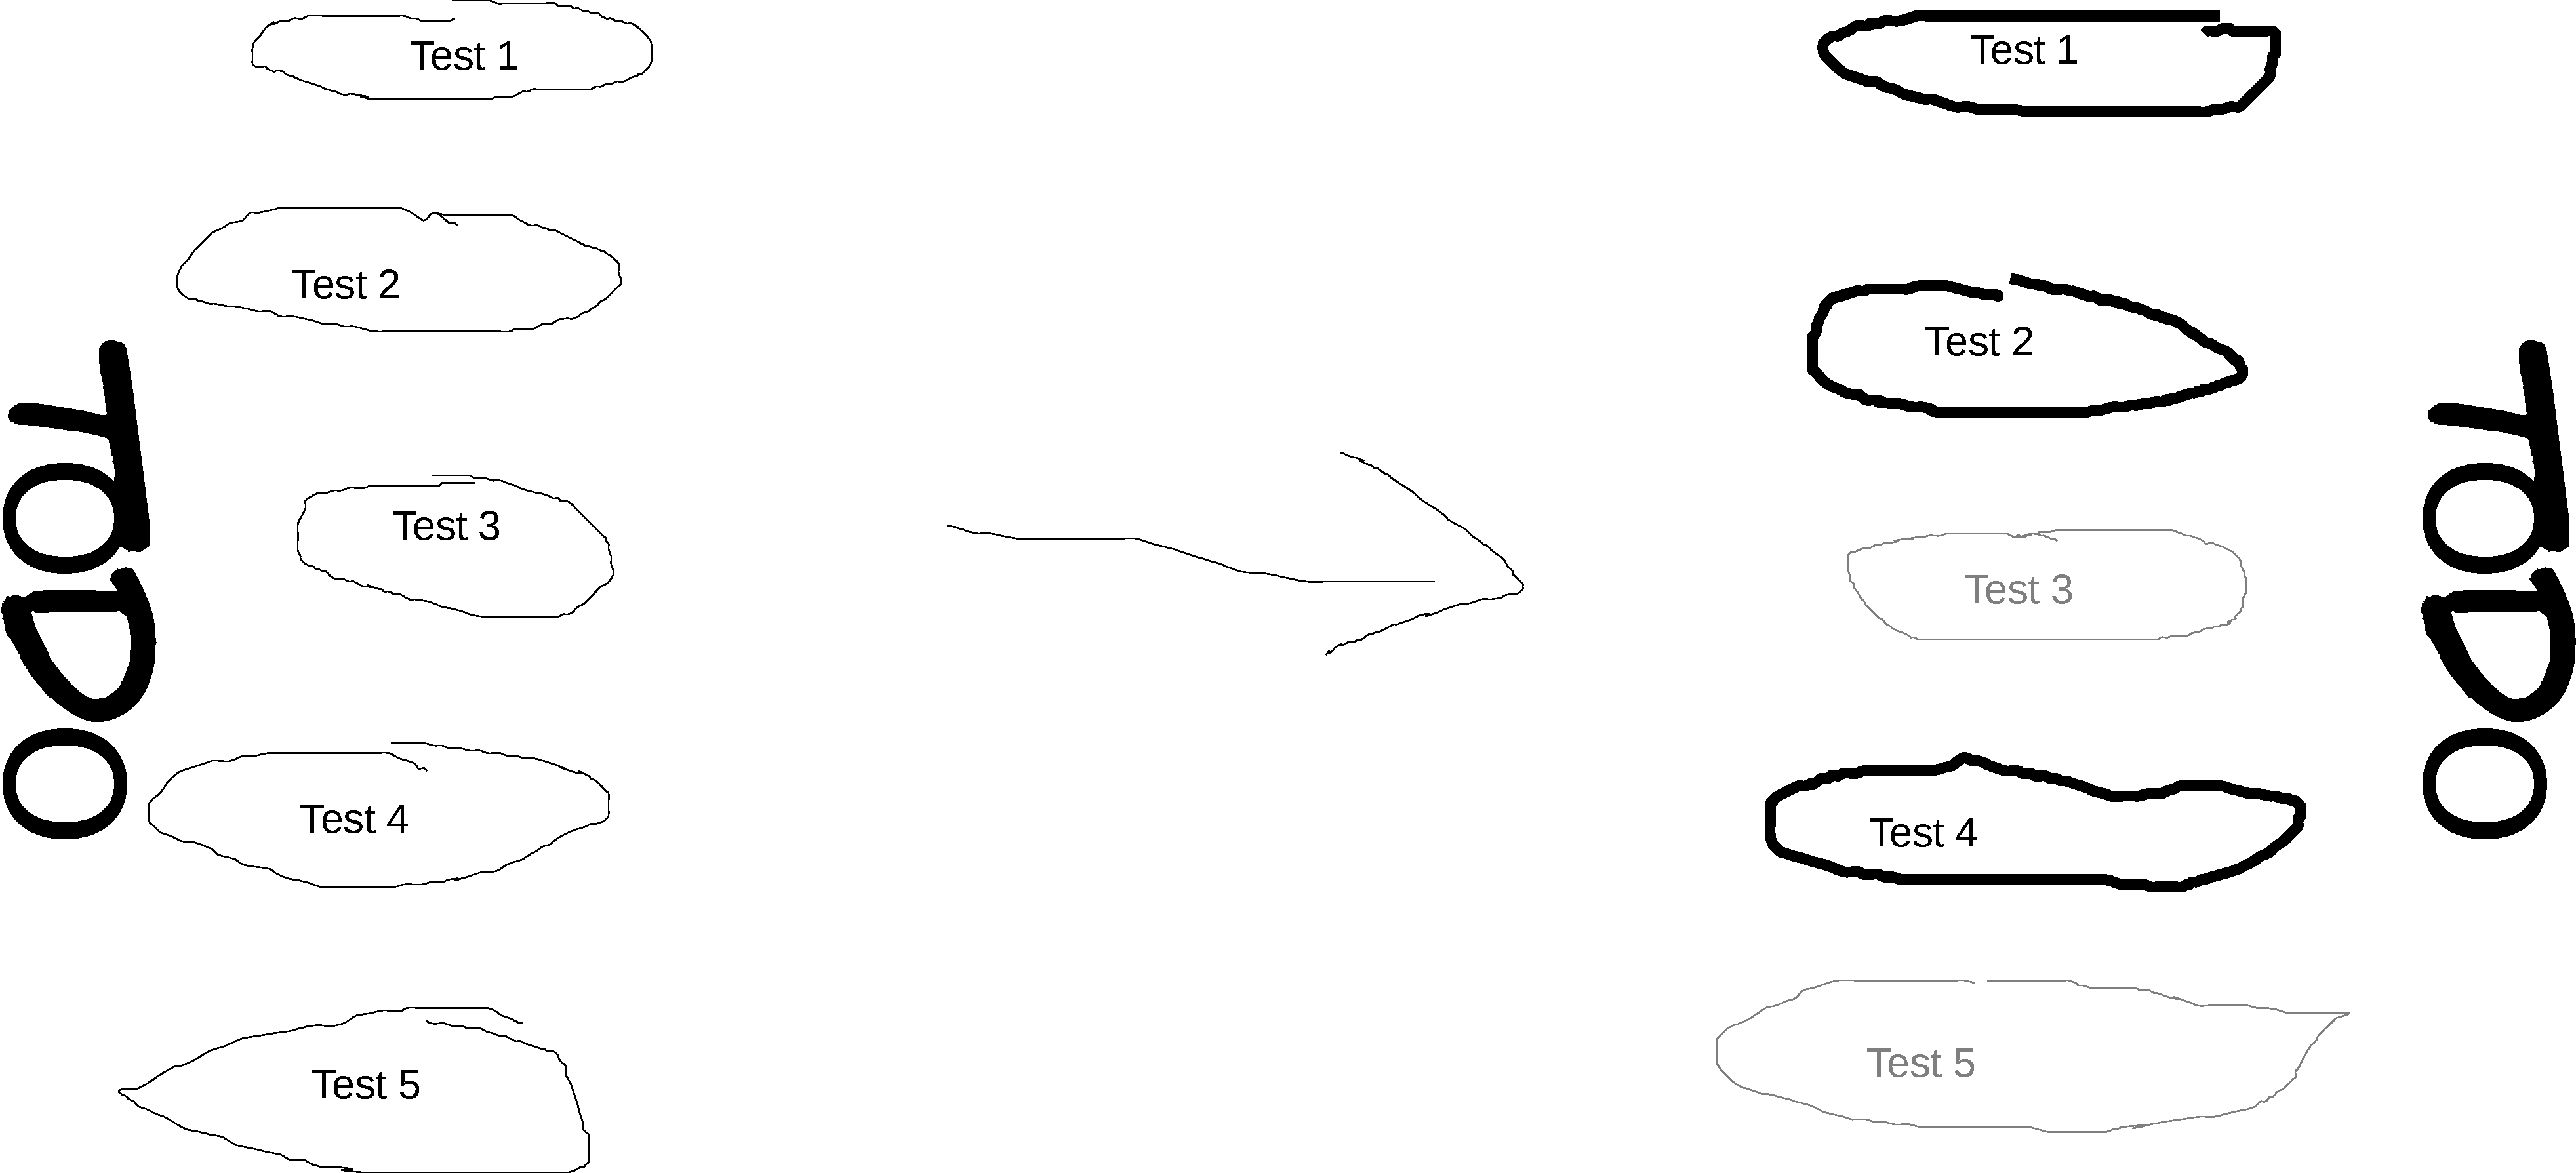
\includegraphics[width=0.8\textwidth]{assets/images/approach-tcs.pdf}
	\caption{\tcs{}}
	\label{fig:tcs}
\end{figure}